\begin{figure}
\begin{center}

\begin{minipage}{\linewidth}
\begin{subfigure}[b]{\linewidth}
\begin{minipage}{0.5\textwidth}
\begin{center}
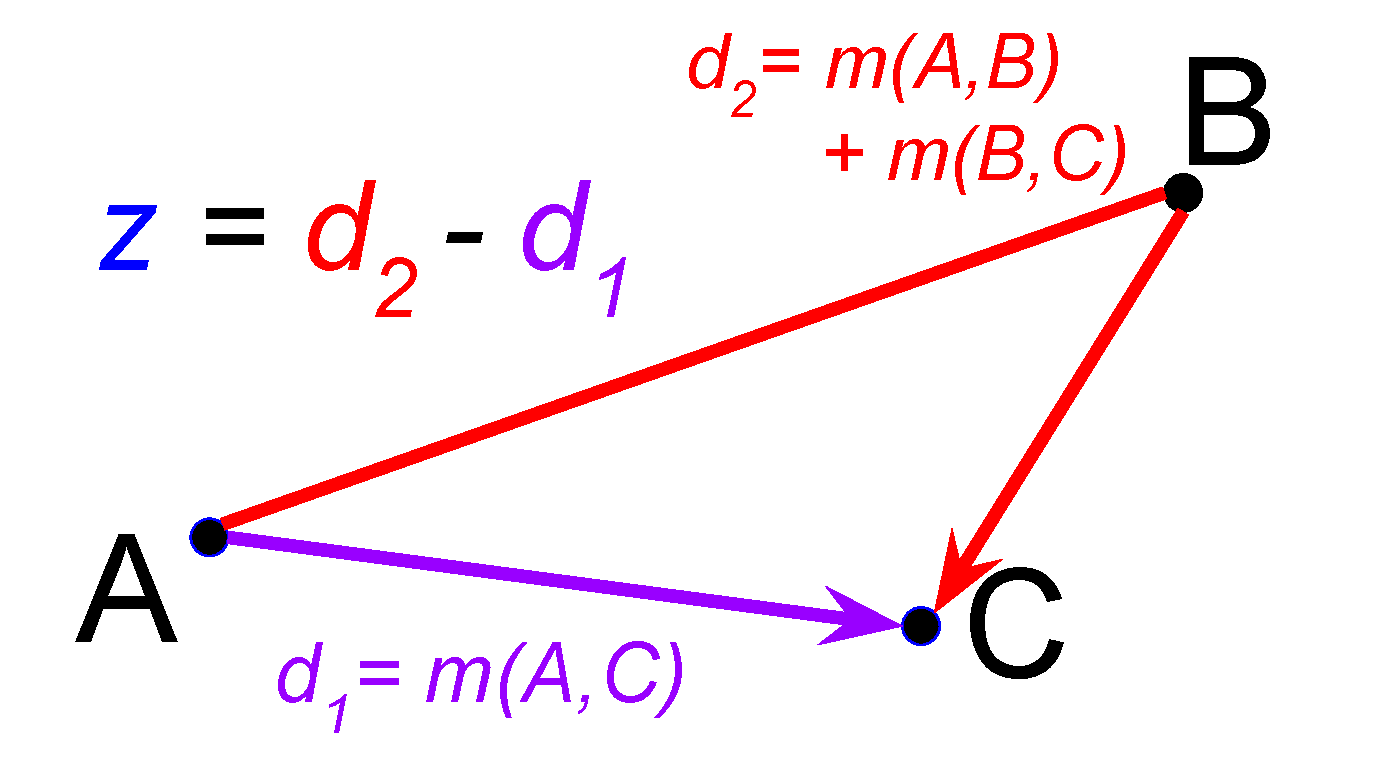
\includegraphics[width=\linewidth,trim=2cm 5cm 2cm 5cm, clip]{img/detour-difference}
\end{center}
\end{minipage}%
\begin{minipage}{0.5\textwidth}
\caption{
Sampling process used to evaluate detour difference, $z$.
} \label{fig:detour_difference_cartoon}
\end{minipage}
\end{subfigure}
\end{minipage}

\begin{minipage}{\linewidth}
\begin{subfigure}[b]{\linewidth}
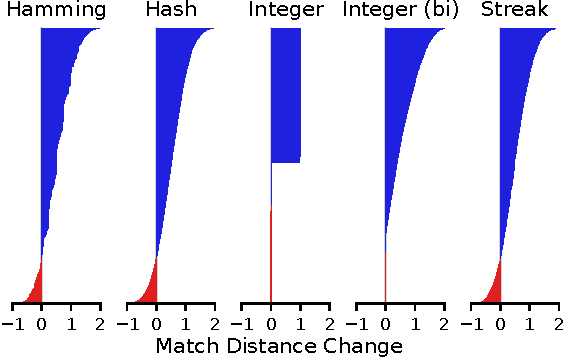
\includegraphics[width=\linewidth]{img/detour_difference/bitweight=0dot5+seed=1+title=low-triplet-analysis+_data_hathash_hash=6b0749ef97a58721+_script_fullcat_hash=297c4fe09078e17b+ext=}
\caption{
Distributions of detour distance difference for triplets of randomly sampled tags.
Each bar sliver represents an independently sampled observation.
A positive value (colored blue) indicates that total distance increased with the addition of an intermediate stop.
A value of exactly 0 indicates an intermediate stop had no effect on total distance.
A negative value (colored red) indicates violation of the triangle inequality: taking an intermediate stop reduced the total distance travelled.
} \label{fig:detour_difference_distribution}

\end{subfigure}
\end{minipage}

\caption{
Detour difference of tag-matching metrics.
}
\label{fig:detour_difference}

\end{center}
\end{figure}
